\documentclass{beamer}

% xcolor and define colors -------------------------
\usepackage{xcolor}

% https://www.viget.com/articles/color-contrast/
\definecolor{purple}{HTML}{5601A4}
\definecolor{navy}{HTML}{0D3D56}
\definecolor{ruby}{HTML}{9a2515}
\definecolor{alice}{HTML}{107895}
\definecolor{daisy}{HTML}{EBC944}
\definecolor{coral}{HTML}{F26D21}
\definecolor{kelly}{HTML}{829356}
\definecolor{cranberry}{HTML}{E64173}
\definecolor{jet}{HTML}{131516}
\definecolor{asher}{HTML}{555F61}
\definecolor{slate}{HTML}{314F4F}

% Mixtape Sessions
\definecolor{picton-blue}{HTML}{00b7ff}
\definecolor{violet-red}{HTML}{ff3881}
\definecolor{sun}{HTML}{ffaf18}
\definecolor{electric-violet}{HTML}{871EFF}

% Main theme colors
\definecolor{accent}{HTML}{00b7ff}
\definecolor{accent2}{HTML}{871EFF}
\definecolor{gray100}{HTML}{f3f4f6}
\definecolor{gray800}{HTML}{1F292D}


% Beamer Options -------------------------------------

% Background
\setbeamercolor{background canvas}{bg = white}

% Change text margins
\setbeamersize{text margin left = 15pt, text margin right = 15pt} 

% \alert
\setbeamercolor{alerted text}{fg = accent2}

% Frame title
\setbeamercolor{frametitle}{bg = white, fg = jet}
\setbeamercolor{framesubtitle}{bg = white, fg = accent}
\setbeamerfont{framesubtitle}{size = \small, shape = \itshape}

% Block
\setbeamercolor{block title}{fg = white, bg = accent2}
\setbeamercolor{block body}{fg = gray800, bg = gray100}

% Title page
\setbeamercolor{title}{fg = gray800}
\setbeamercolor{subtitle}{fg = accent}

%% Custom \maketitle and \titlepage
\setbeamertemplate{title page}
{
    %\begin{centering}
        \vspace{20mm}
        {\Large \usebeamerfont{title}\usebeamercolor[fg]{title}\inserttitle}\\
        {\large \itshape \usebeamerfont{subtitle}\usebeamercolor[fg]{subtitle}\insertsubtitle}\\ \vspace{10mm}
        {\insertauthor}\\
        {\color{asher}\small{\insertdate}}\\
    %\end{centering}
}

% Table of Contents
\setbeamercolor{section in toc}{fg = accent!70!jet}
\setbeamercolor{subsection in toc}{fg = jet}

% Button 
\setbeamercolor{button}{bg = accent}

% Remove navigation symbols
\setbeamertemplate{navigation symbols}{}

% Table and Figure captions
\setbeamercolor{caption}{fg=jet!70!white}
\setbeamercolor{caption name}{fg=jet}
\setbeamerfont{caption name}{shape = \itshape}

% Bullet points

%% Fix left-margins
\settowidth{\leftmargini}{\usebeamertemplate{itemize item}}
\addtolength{\leftmargini}{\labelsep}

%% enumerate item color
\setbeamercolor{enumerate item}{fg = accent}
\setbeamerfont{enumerate item}{size = \small}
\setbeamertemplate{enumerate item}{\insertenumlabel.}

%% itemize
\setbeamercolor{itemize item}{fg = accent!70!white}
\setbeamerfont{itemize item}{size = \small}
\setbeamertemplate{itemize item}[circle]

%% right arrow for subitems
\setbeamercolor{itemize subitem}{fg = accent!60!white}
\setbeamerfont{itemize subitem}{size = \small}
\setbeamertemplate{itemize subitem}{$\rightarrow$}

\setbeamertemplate{itemize subsubitem}[square]
\setbeamercolor{itemize subsubitem}{fg = jet}
\setbeamerfont{itemize subsubitem}{size = \small}







% Links ----------------------------------------------

\usepackage{hyperref}
\hypersetup{
  colorlinks = true,
  linkcolor = accent2,
  filecolor = accent2,
  urlcolor = accent2,
  citecolor = accent2,
}


% Line spacing --------------------------------------
\usepackage{setspace}
\setstretch{1.1}


% \begin{columns} -----------------------------------
\usepackage{multicol}


% Fonts ---------------------------------------------
% Beamer Option to use custom fonts
\usefonttheme{professionalfonts}

% \usepackage[utopia, smallerops, varg]{newtxmath}
% \usepackage{utopia}
\usepackage[sfdefault,light]{roboto}

% Small adjustments to text kerning
\usepackage{microtype}



% Remove annoying over-full box warnings -----------
\vfuzz2pt 
\hfuzz2pt


% Table of Contents with Sections
\setbeamerfont{myTOC}{series=\bfseries, size=\Large}
\AtBeginSection[]{
        \frame{
            \frametitle{Roadmap}
            \tableofcontents[current]   
        }
    }


% Tables -------------------------------------------
% Tables too big
% \begin{adjustbox}{width = 1.2\textwidth, center}
\usepackage{adjustbox}
\usepackage{array}
\usepackage{threeparttable, booktabs, adjustbox}
    
% Fix \input with tables
% \input fails when \\ is at end of external .tex file
\makeatletter
\let\input\@@input
\makeatother

% Tables too narrow
% \begin{tabularx}{\linewidth}{cols}
% col-types: X - center, L - left, R -right
% Relative scale: >{\hsize=.8\hsize}X/L/R
\usepackage{tabularx}
\newcolumntype{L}{>{\raggedright\arraybackslash}X}
\newcolumntype{R}{>{\raggedleft\arraybackslash}X}
\newcolumntype{C}{>{\centering\arraybackslash}X}

% Figures

% \imageframe{img_name} -----------------------------
% from https://github.com/mattjetwell/cousteau
\newcommand{\imageframe}[1]{%
    \begin{frame}[plain]
        \begin{tikzpicture}[remember picture, overlay]
            \node[at = (current page.center), xshift = 0cm] (cover) {%
                \includegraphics[keepaspectratio, width=\paperwidth, height=\paperheight]{#1}
            };
        \end{tikzpicture}
    \end{frame}%
}

% subfigures
\usepackage{subfigure}


% Highlight slide -----------------------------------
% \begin{transitionframe} Text \end{transitionframe}
% from paulgp's beamer tips
\newenvironment{transitionframe}{
    \setbeamercolor{background canvas}{bg=accent!40!black}
    \begin{frame}\color{accent!10!white}\LARGE\centering
}{
    \end{frame}
}


% Table Highlighting --------------------------------
% Create top-left and bottom-right markets in tabular cells with a unique matching id and these commands will outline those cells
\usepackage[beamer,customcolors]{hf-tikz}
\usetikzlibrary{calc}
\usetikzlibrary{fit,shapes.misc}

% To set the hypothesis highlighting boxes red.
\newcommand\marktopleft[1]{%
    \tikz[overlay,remember picture] 
        \node (marker-#1-a) at (0,1.5ex) {};%
}
\newcommand\markbottomright[1]{%
    \tikz[overlay,remember picture] 
        \node (marker-#1-b) at (0,0) {};%
    \tikz[accent!80!jet, ultra thick, overlay, remember picture, inner sep=4pt]
        \node[draw, rectangle, fit=(marker-#1-a.center) (marker-#1-b.center)] {};%
}

\usepackage{breqn} % Breaks lines

\usepackage{amsmath}
\usepackage{mathtools}

\usepackage{pdfpages} % \includepdf

\usepackage{listings} % R code
\usepackage{verbatim} % verbatim

% Video stuff
\usepackage{media9}

% packages for bibs and cites
\usepackage{natbib}
\usepackage{har2nat}
\newcommand{\possessivecite}[1]{\citeauthor{#1}'s \citeyearpar{#1}}
\usepackage{breakcites}
\usepackage{alltt}

% Setup math operators
\DeclareMathOperator{\E}{E} \DeclareMathOperator{\tr}{tr} \DeclareMathOperator{\se}{se} \DeclareMathOperator{\I}{I} \DeclareMathOperator{\sign}{sign} \DeclareMathOperator{\supp}{supp} \DeclareMathOperator{\plim}{plim}
\DeclareMathOperator*{\dlim}{\mathnormal{d}\mkern2mu-lim}
\newcommand\independent{\protect\mathpalette{\protect\independenT}{\perp}}
   \def\independenT#1#2{\mathrel{\rlap{$#1#2$}\mkern2mu{#1#2}}}
\newcommand*\colvec[1]{\begin{pmatrix}#1\end{pmatrix}}

\newcommand{\myurlshort}[2]{\href{#1}{\textcolor{gray}{\textsf{#2}}}}


\begin{document}

\imageframe{./lecture_includes/mixtape_did_cover.png}


% ---- Content ----

\section{Imputation DiD}

\subsection{Imputation based robust estimator}



\begin{frame}{Background}

\begin{itemize}

\item The origin of the robust diff-in-diff papers identifying pathologies in TWFE was Borusyak and Jaravel (2016) working paper
\item Both problems with static and dynamic specifications were discussed, and the identification of the ``already treated'' as controls
\item Paper remained in working paper until 2021 when Jan Speiss was brought on; the team developed a new estimator
\item We will focus primarily on the estimator, to avoid redundancies

\end{itemize}

\end{frame}

\begin{frame}{My Outline}

\begin{enumerate}
\item Discussion of their interpretation of ``basic'' DiD assumptions
\item Critique of TWFE OLS when strong assumptions don't hold
\item Introduction of new assumptions
\item Robust efficient imputation estimator
\end{enumerate}

\end{frame}


\begin{frame}{ATT parameter}

Estimation target will be unit level treatment effects aggregated to a higher level like the ATT:

\begin{eqnarray*}
\tau_w = \sum_{it \in \Omega_{1}}w_{it}\tau_{it} = w'_1\tau
\end{eqnarray*}

\bigskip

Note the weights -- they need not add up to one.  Weights could be $\frac{1}{N}$ for all $it \in \Omega_1$. We have a number of options. 


\end{frame}

\begin{frame}{Standard TWFE Assumptions}

\begin{enumerate}
\item Parallel trends -- expressed as a TWFE model
\item No anticipation
\item Homogenous treatment effects
\end{enumerate}

\end{frame}

\begin{frame}{A1: Parallel trends}

\textbf{Assumption 1: Parallel trends}. There exist non-stochastic $\alpha_i$ and $\beta_t$ such that:

$$Y_{it}(0) = \alpha_i + \beta_t + \varepsilon_{it}$$with $$E[\varepsilon_{it}]=0$$for all $it \in \Omega$. Can be extended (e.g., unit-specific trends). Only imposes restrictions on $Y(0)$, not treatment effects themselves. Notice how it is a TWFE assumption -- it's actually the same data generating process as in baker.do.

\end{frame}

\begin{frame}{A2: No anticipation}

\begin{itemize}
\item No anticipation rules out anticipatory behavior that would cause treatment effects to materialize even before the treatment occurred:$$Y_{it} = Y_{it}(0)$$ for all $it \in \Omega_0$. 
\item Notice how as an assumption, it literally imposes $\tau=0$ for all pre-treatment periods. 

\end{itemize}

\end{frame}

\begin{frame}{A2: No anticipation}

\begin{itemize}
\item Caveat: No Anticipation was never mentioned until recently
\item It's crucial for the pre-trends to be zero, far more than parallel trends, as parallel trends is \emph{only} about post-treatment from baseline, whereas event studies are about pre-trends and that's where no anticipation reigns
\end{itemize}

\end{frame}


\begin{frame}{A3: Restricted causal effects}

This is the one that places restrictions on what treatment effects can and cannot be (i.e., homogenous treatment effects). Notice the very detailed expression:

\bigskip

\textbf{Assumption 3 (Restricted causal effects)}: $B\tau0$ for a known $M \times N_1$ matrix $B$ of full row rank. 

\bigskip

If we can assume something like homogenous treatment effects, then TWFE actually is best because its ability to \emph{correctly} extrapolate will increase efficiency. But it's when A3 is not tenable or not really ex ante justified by theory that we should be worried. There's an A3' that is a slight modification. 

\end{frame}


\begin{frame}{Critique of Common Practice}

\begin{enumerate}
\item Under-identification in event studies
\item Negative weighting
\item Spurious identification of long-run casual effects
\end{enumerate}

\end{frame}

\begin{frame}{Critique: Underidentification problem}


\textbf{Lemma 1}: If there are no never-treated units, the path of [pre-treatment lead population regression coefficients] is not point identified in the fully dynamic OLS specification.  In particular. adding a linear trend to this path $\{\tau_h + k(h+1) \}$ for any $k \in R$ fits the data equally well with the fixed effects coefficients appropriately modified.

\bigskip

In english, it means you're going to have a multicollinearity problem even worse than you thought when estimating the fully dynamic event study model (i.e., dropping only one lead for all base comparisons)

\end{frame}


\begin{frame}{Underidentification of lead coefficients}

\begin{block}{Under-identification problem}
Formally the problem arises because a linear time trend $t$ and a linear term in the cohort $E_i$ (subsumed by the unit FEs) can perfectly reproduce a linear term in relative time $K_{it}=t-E_i$.  Therefore a complete set of treatment leads and lags, which is equivalent to the FE of relative time, is collinear with the unit and period FEs.
\end{block}

\bigskip

Just one additional normalization is needed -- drop $\tau_{-a}=0$ and $\tau_{-1}=0$.  This will break the multicollinearity.  We saw this in SA also.  So multiple people saw this at the same time.

\end{frame}

\begin{frame}{Under-identification and theoretical justifications}

\begin{itemize}
\item Imposing any $-a$ lead and $-1$ lead to equal zero is somewhat ad hoc.  Why those two and not some other two?
\item Recall with SA -- it mattered which ones you dropped because otherwise leads were contaminated
\item This is again about NA -- if you chose $-a$ and $-1$, then you had some theoretical reason to assume NA held for them and not some other periods
\end{itemize}

\end{frame}



\begin{frame}{Negative weighting and violations of A3}

Assume some simple static model with a single dummy for treatment.  Then they lay out a second lemma

\bigskip 
\textbf{Lemma 2}: If A1 and A2 hold, then the estimand of the static OLS specification satisfies $\tau^{static}=\sum_{it \in \Omega_1} w_{it}^{OLS}\tau_{it}$ for some weights $w_{it}^{OLS}$ that do not depend on the outcome realizations and add up to one $\sum_{it \in \Omega_1}=1$.

\bigskip

The static OLS estimand cannot be interpreted as a ``proper'' weighted average, as some weights can be negative. 

\end{frame}


\begin{frame}{Simple illustration}


\begin{table}[htb]\centering
\scriptsize
\caption{TWFE dynamics}
\centering
\begin{threeparttable}
\begin{tabular}{l*{2}{c}}
\toprule
\multicolumn{1}{l}{$E(y_{it})$ }&
\multicolumn{1}{c}{\textbf{$i=A$ }}&
\multicolumn{1}{c}{\textbf{$i=B$ }}\\
\midrule
t=1 & $\alpha_A$ & $\alpha_B$ \\
t=2 & $\alpha_A + \beta_2 + \delta_{A2}$ & $\alpha_B$ + $\beta_2$ \\
t=3 & $\alpha_A + \beta_3 + \delta_{A3}$ & $\alpha_B$ + $\beta_3$ + $\delta_{B3}$ \\
\midrule
Event date & $E_i=2$ & $E_i = 3$ \\
\bottomrule
\end{tabular}
\end{threeparttable}
\end{table}

Static: $\delta = \delta_{A2} + \frac{1}{2}\delta_{B3} - \frac{1}{2} \delta_{A3}$.  \\

\bigskip

Notice the negative weight on the furthest lag. This is what you get when A3 is not satisfied.. 

\end{frame}


\begin{frame}{Short-run bias of TWFE}

\begin{itemize}
\item TWFE OLS has a severe short-run bias
\item the long-run causal effect, corresponding to the early treated unit A and the late period 3, enters with a negative weight (-1/2)
\item The larger the effects in the long-run, the smaller the coefficient will be
\item It's caused by ``forbidden comparisons'' (late to early treated) -- we saw this with Goodman-Bacon (2021)
\item Forbidden comparisons create downward bias on long-run effects with treatment effect heterogeneity, \emph{but not with treatment effect homogeneity} -- so it really is an A3 violation
\end{itemize}

\end{frame}

\begin{frame}{Spurious Long-Run Causal Effects}

More A3 problems, this time finding long-run effects  where there are none. Basically, you need to impose a lot of pre-trend restrictions to get estimates of long-run population regression coefficients. Even then you can't get them all. 

\bigskip

OLS estimates are fully driven by unwarranted extrapolations of treatment effects across observations and may not be trusted unless strong ex ante justifications for A3 exist

\bigskip

\textbf{Lemma 4}: Suppose there are no never-treated units and let $H=max_i E_i - min_i E_i$. Then for any non-negative weights $w_{it}$ defined over the set of observations with $K_{it} \geq \overline{H}$ (that are not identically zero), the weighted sum of causal effects $\sum_{it:K_{it}\geq \overline{H}}w_{it} \tau_{it}$ is not identified by A1 and A2.

\end{frame}

\begin{frame}{Modifications of general model}


Modification of A1 to A1': $$ Y_{it}(0) = A'_{it} \lambda_i + X_{it}' \delta + \varepsilon_{it}$$

\bigskip

Assumption 4 is introduced (homoskedastic residuals).  This is key, because they will be building an ``efficient estimator'' with BLUE like OLS properties. 

\bigskip

Using A1' to A4, we get the ``efficient estimator'' which is for all linear unbiased estimates of $\delta_W$, the unique efficient estimator $\widehat{\delta_W^*}$ can be obtained with 3 steps

\end{frame}


\begin{frame}{Role of the untreated observations}

\begin{quote}
``At some level, all methods for causal inference can be viewed as imputation methods, although some more explicitly than others.'' -- Imbens and Rubin (2015)
\end{quote}

\bigskip

\begin{quote}
``The idea is to estimate the model of $Y_{it}^0$ using the untreated observations and extrapolate it to impute $Y_{it}^0$ for treated observations.''
\end{quote}


\end{frame}

\begin{frame}{Steps}

\begin{enumerate}
\item Estimate expected potential outcomes using OLS and only the untreated observations (this is similar to Gardner 2021)
\item Then calculate $\widehat{\delta}_{it} = Y_{it}^1 - \widehat{Y}_{it}^0$
\item Then estimate target parameters as weighted sums$$\widehat{\delta}_W = \sum_{it}w_{it}\widehat{\delta}_{it}$$
\end{enumerate}

\end{frame}


\begin{frame}{Why is this working?}

\begin{itemize}
\item Think back to that original statement of the PT assumption -- you're modeling $Y(0)_{it}$. 
\item That is, without treatment -- so the potential outcomes do not depend on any treatment effect
\item Hence where we get treatment heterogeneity
\item We obtain consistent estimates of the fixed effects which are then used to extrapolate to the counterfactual units for all $Y(0)_{it \in \Omega_1}$
\item I think this is a very cool trick personally, and as it is still OLS, it's computationally fast and flexible to unit-trends, triple diff, covariates and so forth (though remember what we said about covariates)
\end{itemize}

\end{frame}


\begin{frame}{Comparisons to other estimators}

\begin{center}
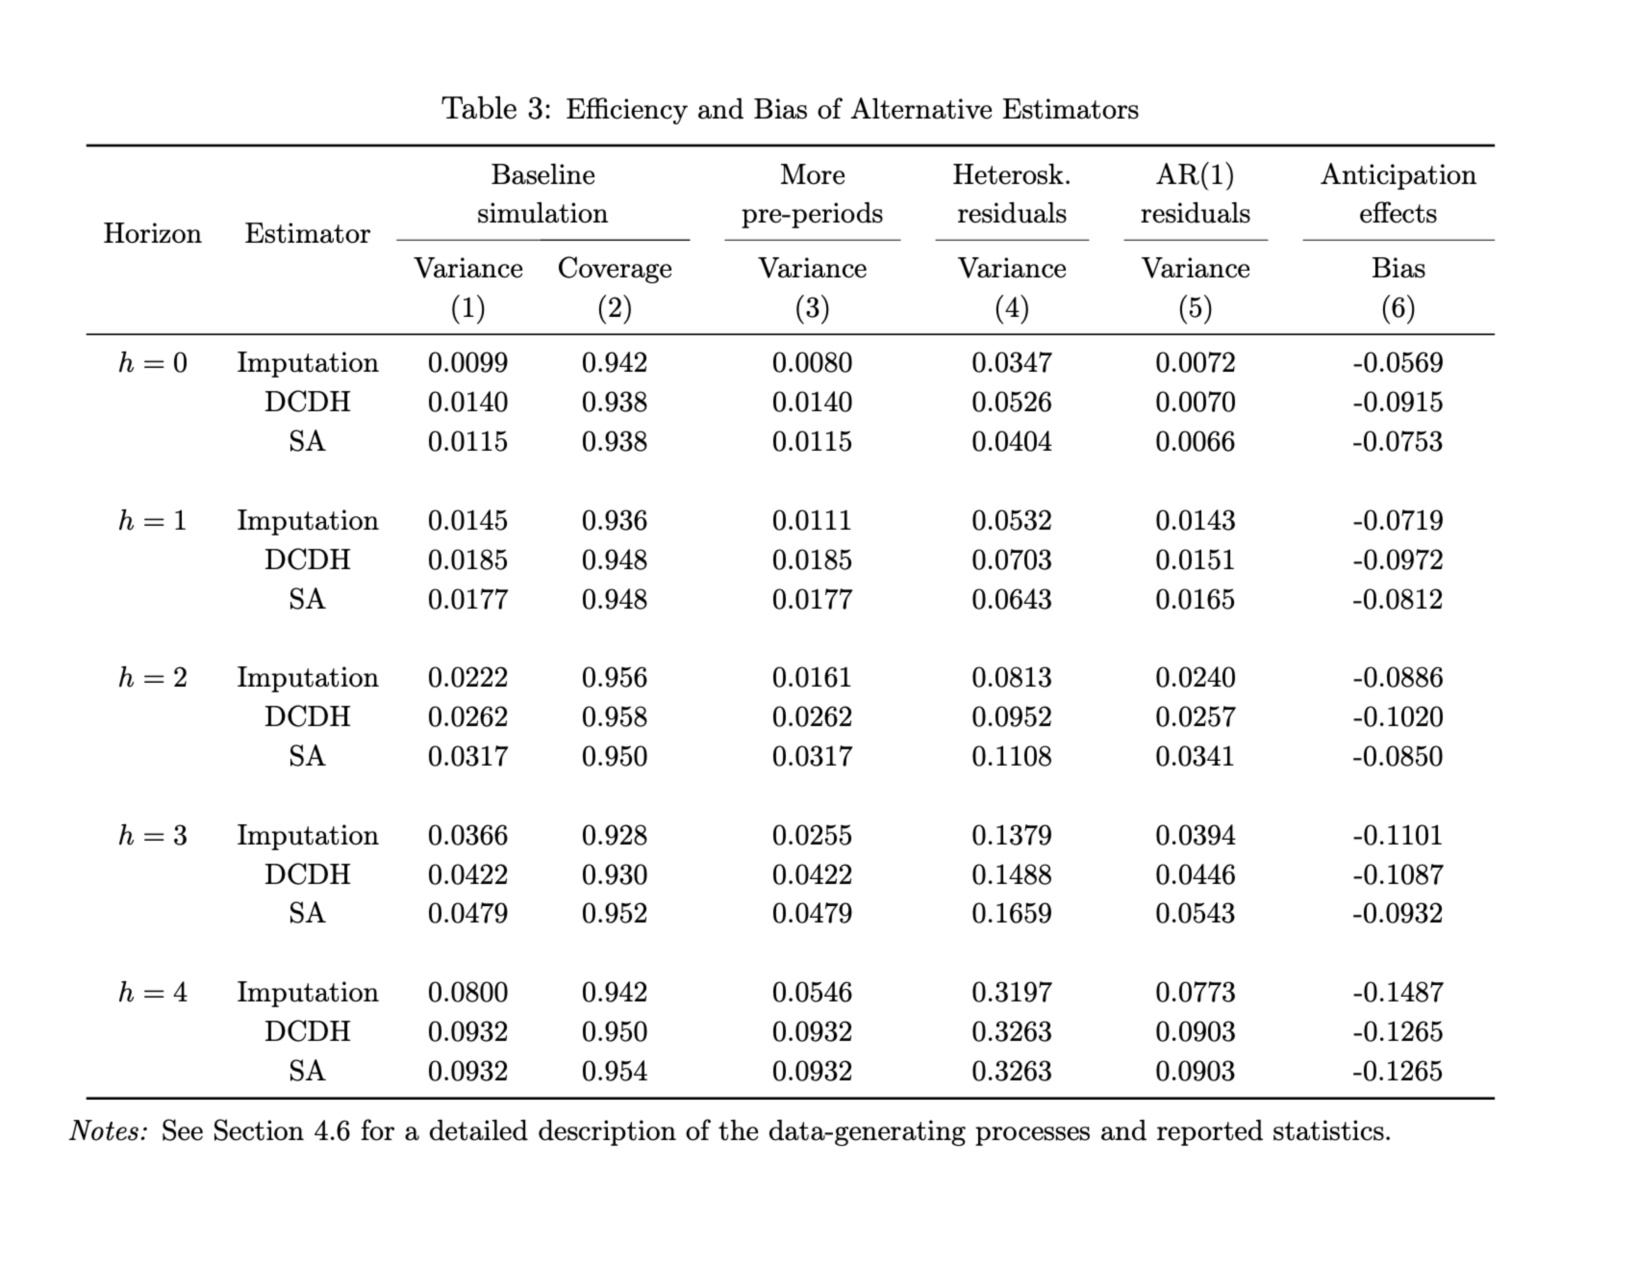
\includegraphics[scale=0.35]{./lecture_includes/bjs_sim.pdf}
\end{center}

\end{frame}

\begin{frame}{Returning to the minimum wage}

\begin{itemize}
\item Clemens and Strain (2021) implemented the BJS imputation estimator to estimate the effect of the minimum wage (post Great Recession) on employment
\item One comment abt the following graphics: BJS procedure does not have a ``base'' period in the same sense as the regression models do because it is not contrasting each period relative to some omitted group
\item Since it is imputing counterfactuals, we can calculate each period's effect
\end{itemize}

\end{frame}

\begin{frame}{BJS Results}

	\begin{figure}
	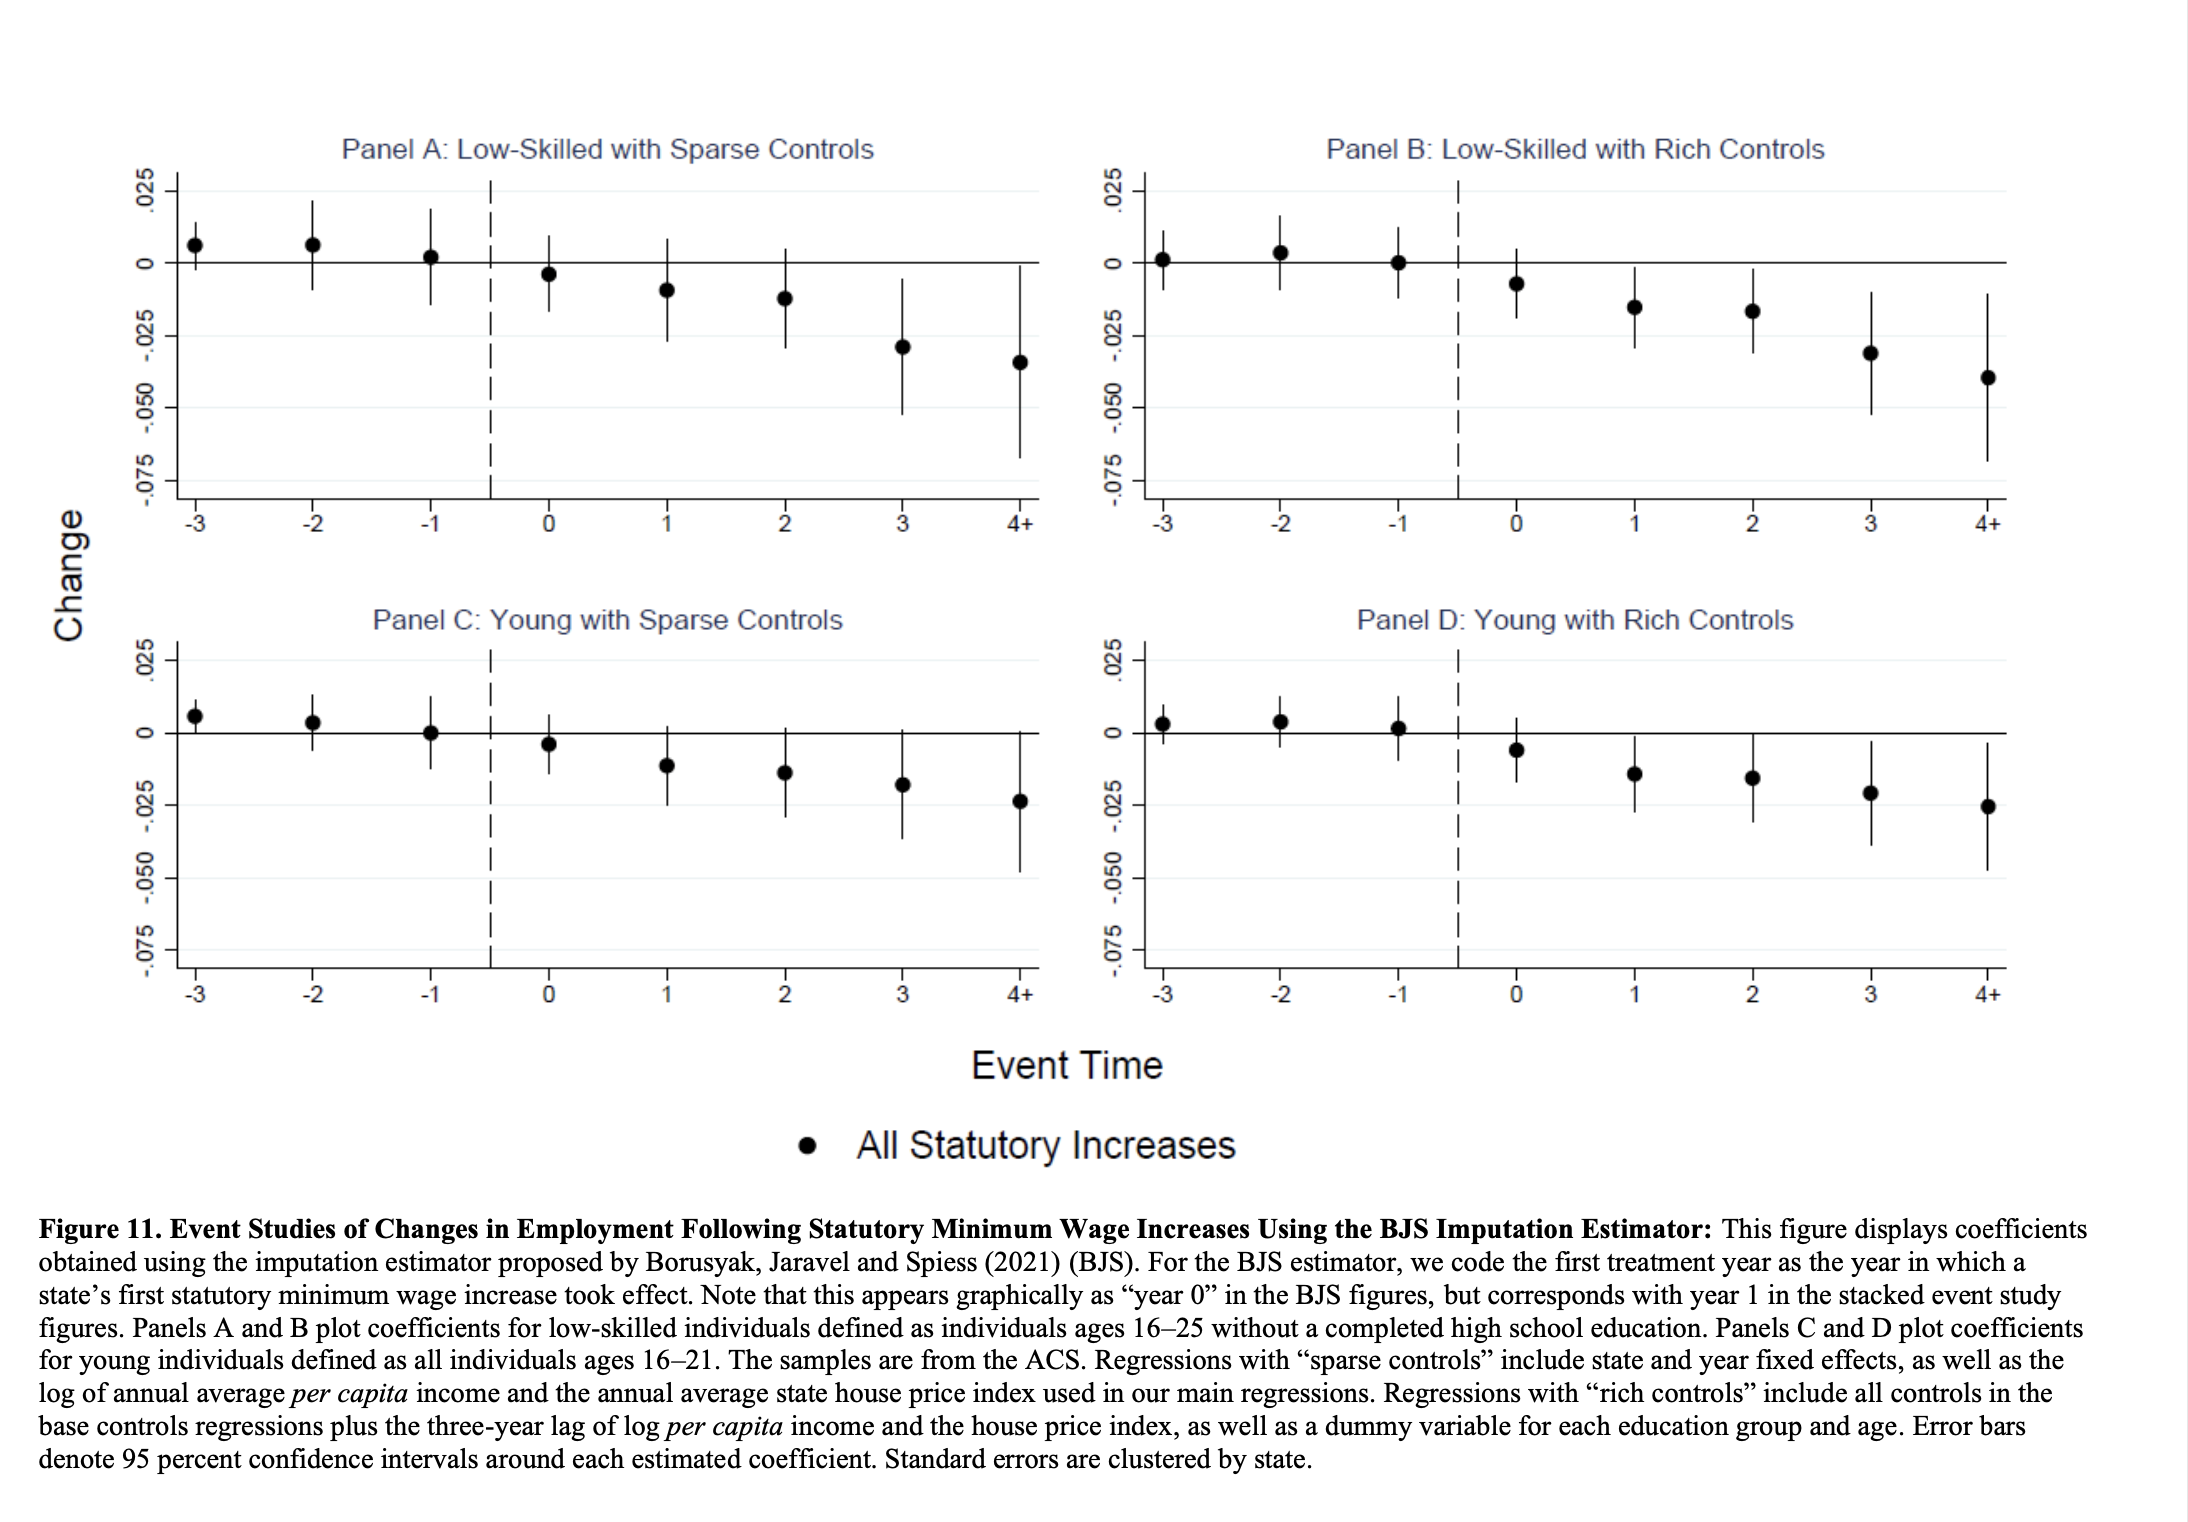
\includegraphics[scale=0.25]{./lecture_includes/Clemens_bjs_1.png}
	\end{figure}

\end{frame}

\begin{frame}{BJS Results}

	\begin{figure}
	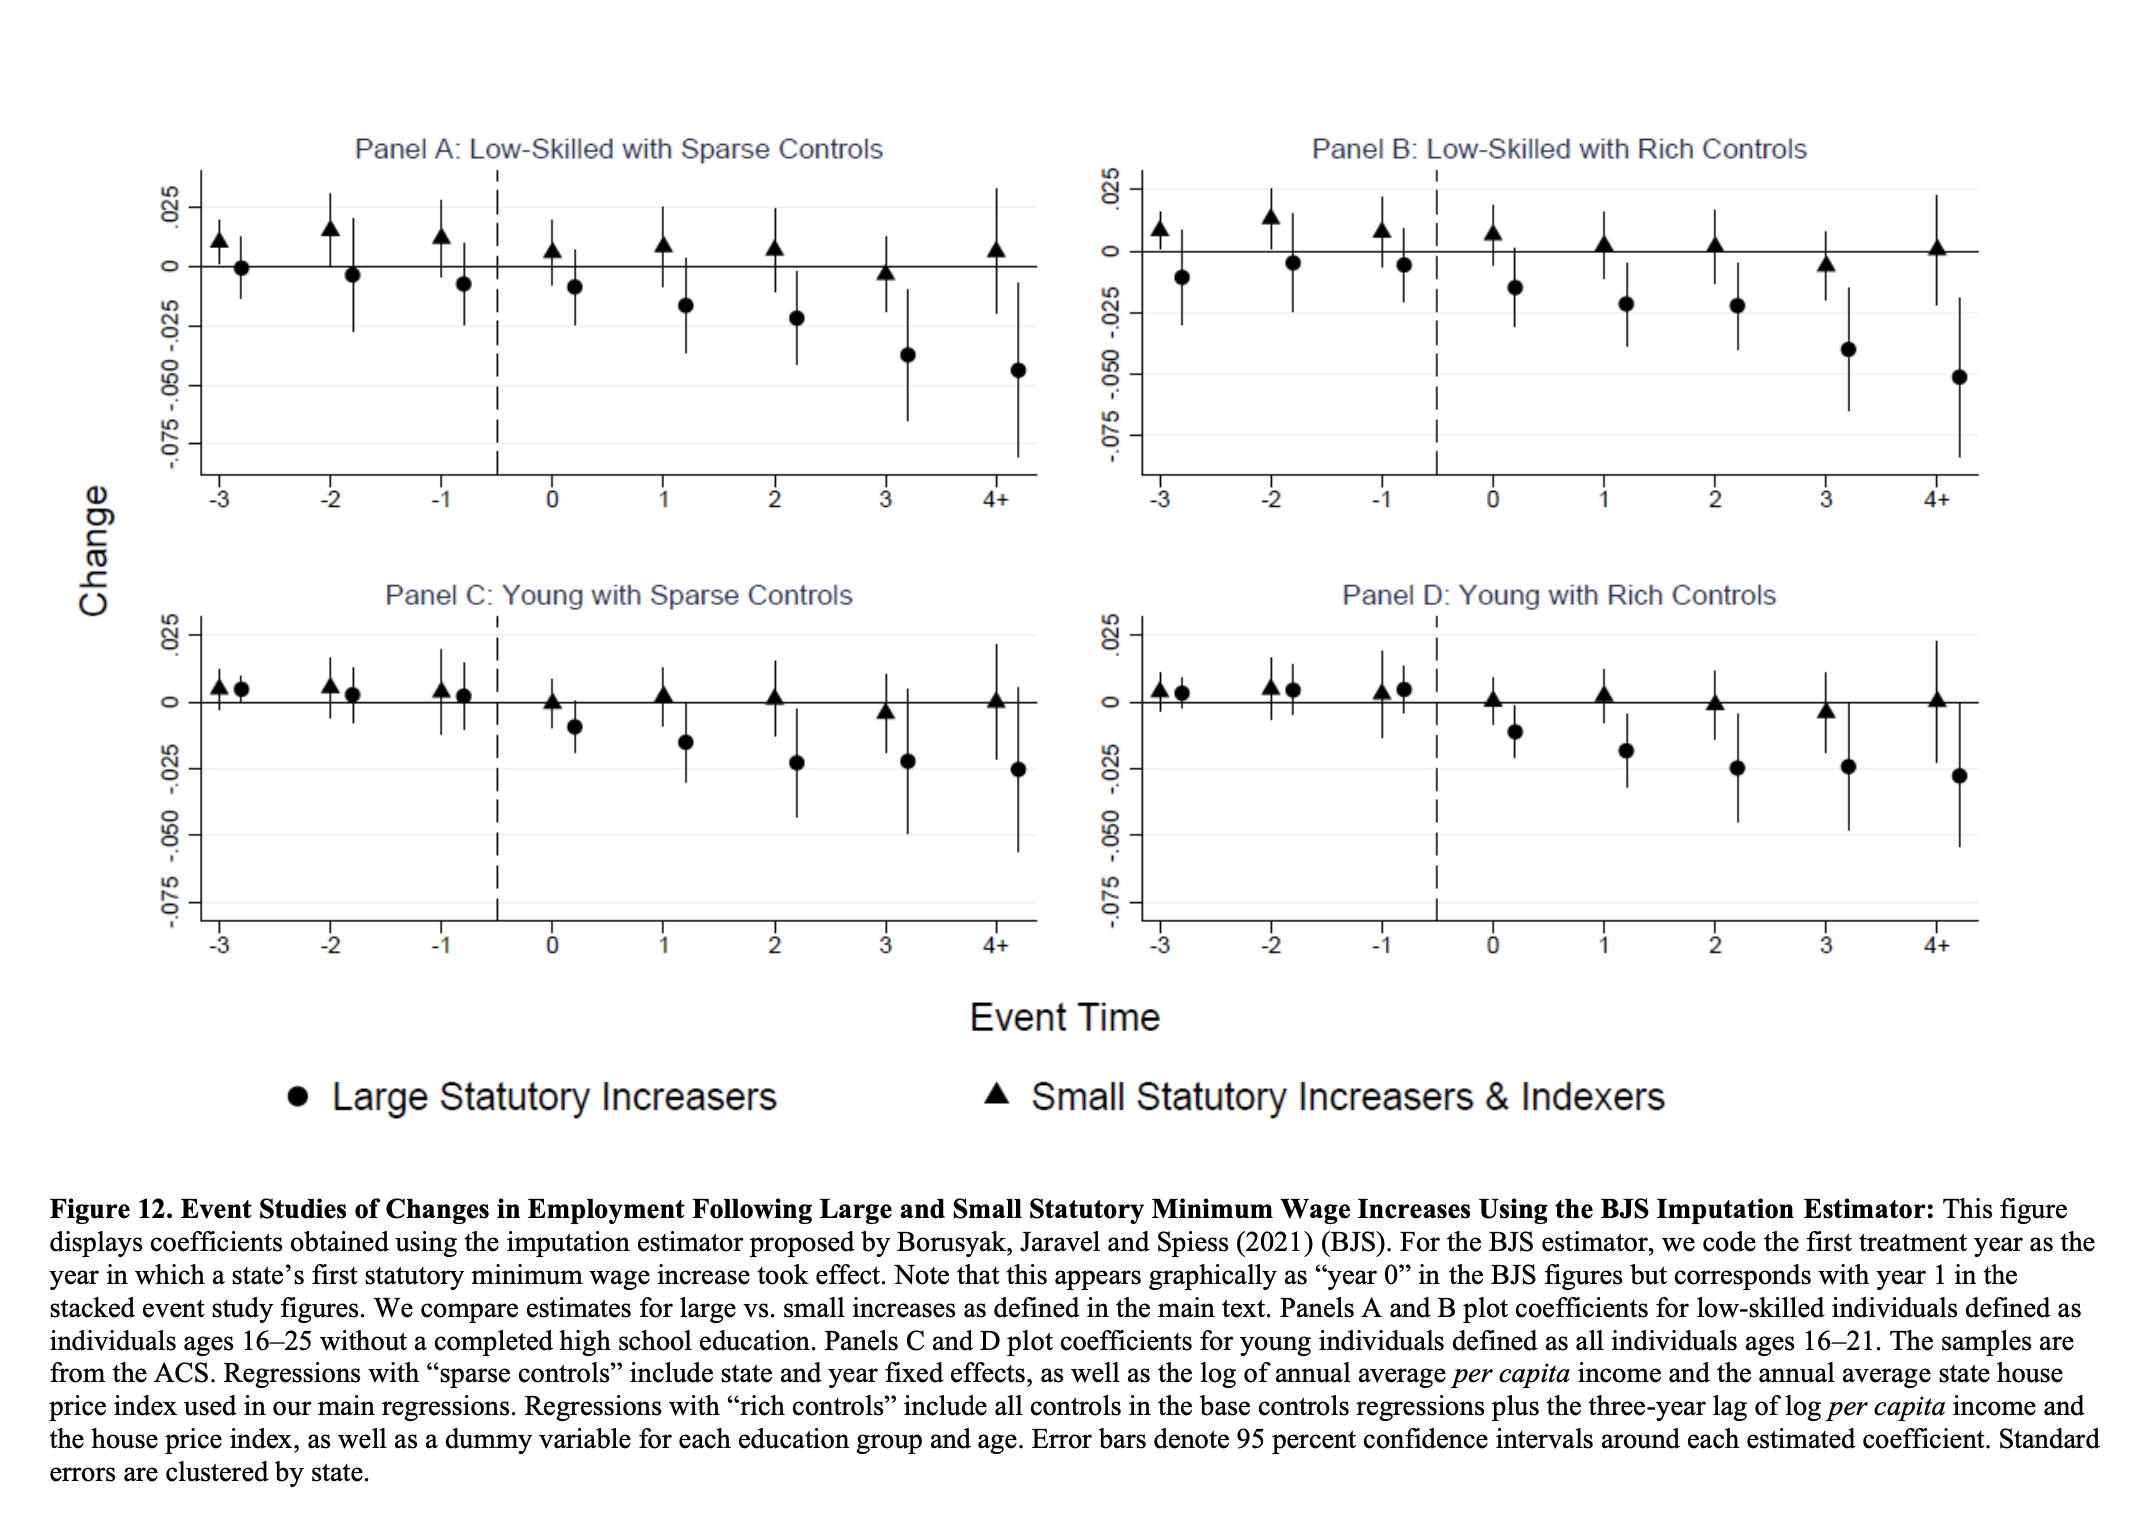
\includegraphics[scale=0.25]{./lecture_includes/Clemens_bjs_2.png}
	\end{figure}

\end{frame}

\begin{frame}{Comments abt the minimum wage study}

\begin{itemize}
\item Elasticity of employment with respect to minimum wage is -0.124 and -0.082 for those without high school and the young, respectively
\item Differences by size of minimum wage increase:
	\begin{itemize}
	\item Large increases (around \$2.90): own-wage elasticity is -1.01 for 16-25yo with less than HS and -0.41 for 16 to 21yo (large effects)
	\item Small increases (around \$1.90): own-wage elasticity is 0.46 (i.e., no employment effects)
	\item Inflation-index increases (around \$0.90): own-wage elasticity is 0.16 (no effect) and -0.17 (no effect)
	\end{itemize}
\end{itemize}

\end{frame}

\subsection{2SDiD}

\begin{frame}{Two Stage DiD}

\begin{quote}
``It seems natural that TWFE should identify the ATT'' -- Gardner (2021)
\end{quote}

\bigskip

It just seems like TWFE with a DiD will estimate the ATT with weights that we'll find intuitive.  Was this just a conjecture and was never true?  Why isn't this working?

\end{frame}



\begin{frame}{Two Stage DiD}

\begin{itemize}
\item Why does TWFE fail under differential timing? Violates strict exogeneity under heterogeneity
\item The logic of the failure suggests an obvious, but previously unknown, solution which is the 2SDiD
\item I'll explain 2SDiD, focus on the parallel trends implications, and show we can get a consistent and unbiased estimate of group and relative time fixed effects
\item If you can get consistent and unbiased estimates of group and relative time fixed effects, then you can delete them and run normal analysis
\end{itemize}

\end{frame}

\begin{frame}{Background}

\begin{itemize}
\item By now, we all agree that TWFE just doesn't handle heterogeneity under differential timing very well
\item We've seen in the Goodman-Bacon decomposition why -- it's caused by TWFE implicitly calculating late to early 2x2s, which are a source of bias
\item But some of you are coming straight from a panel econometrics course that maybe didn't use potential outcomes notation
\item Isn't strict exogeneity enough for consistent estimates?  What then does strict exogeneity have to do with heterogeneity and differential timing?
\end{itemize}

\end{frame}

\begin{frame}{High level discussion}

\begin{itemize}
\item TWFE identifies the ATT when the heterogeneous effects are distributed equally across all groups and periods, but since that is a knife-edge situation, it is likely that TWFE will not in our applications meet this special scenario
\item In the two group case, that is what happens though which is why TWFE worked fine there
\item Metaphorically, the two group case that we always used to pin our intuition of what DiD was doing was the exception not the rule
\item Goodman-Bacon (2021) shows the problem is caused by late-to-early comparisons; Gardner (2021) will show that the problem is misspecification
\item Think of these as different perspectives on the same problem
\end{itemize}

\end{frame}

\begin{frame}{Model misspecification}

\begin{quote}
``Misspecified DiD regression models project heterogenous treatment effects onto group and period fixed effects rather than the treatment status itself''
\end{quote}

\bigskip

Spoiler: This analysis of the problem suggests solution -- why don't we remove those?

\end{frame}


\begin{frame}{2SDiD}

\begin{itemize}
\item First stage -- estimate the group and relative time fixed effects using only the $D=0$ observations
\item Second stage -- using predicted values based off those fixed effect coefficients, run your model off the transformed outcome 
\item Get the standard errors right just like 2SLS by taking the first stage into account (uses GMM)
\end{itemize}

\end{frame}

\begin{frame}{More high level}

\begin{itemize}
\item The second step recovers the average difference in outcomes between treated and untreated units after removing group and period fixed effects
\item Strong parallel trends assumption compared to CS and SA, but unclear if this is a big deal in general
\end{itemize}

\end{frame}

\begin{frame}{Notation}

$i$: panel units \\
$t$: calendar time -- think of real dates\\
$g\in \{0,1, \dots , G \}$ -- groups\\
$p \in \{0,1, \dots , P \}$  -- relative time or ``periods''\\

\bigskip

Periods are successive.  Group 0 -- never treated. Group 1 -- treated in period 1, 2, and on.  Group 2 -- treated in period 2, etc.

\end{frame}

\begin{frame}{Parameters}

\begin{eqnarray*}
\beta_{gp} = E \bigg [ Y^1_{gpit} - Y^0_{gpit} | g,p \bigg ]
\end{eqnarray*}

\bigskip

It's a group-time ATT but expressed in a more traditional econometric notation that you could easily find in Wooldridge or some such

\end{frame}

\begin{frame}{Modeling basics}

Under parallel trends, mean outcomes will satisfy the following equation

\bigskip

\begin{eqnarray*}
E \bigg [ Y_{gpit} | g,p,D_{gp} \bigg ] = \lambda_g + \gamma_p + \beta_{gp} D_{gp}
\end{eqnarray*}

\bigskip

In two-group, group and period effects are eliminated with dummies because TWFE uses dummies to demean across multiple dimensions. Then TWFE identifies ATT.  But this does not hold when average effects vary across group and period. There are many ways to express a treatment effect's across group and time, but Gardner presented it as a weighted average of the coefficients for only that group-period situation:

\begin{eqnarray*}
E \bigg (\beta_{gp} | D_{gp}=1 \bigg ) = E \bigg (Y^1_{gpit} - Y^0_{gpit} | D_{gp}=1 \bigg )
\end{eqnarray*}

\end{frame}


\begin{frame}{Strict exogeneity violation}

Rewriting the above we get:

\begin{eqnarray*}
E \bigg [ Y_{gpit} | g,p, D_{gp} \bigg ] &=& \lambda_g + \gamma_p + E \bigg [\beta_{gp} | D_{gp} =1 \bigg ] D_{gp} \\
&& \bigg [\beta_{gp} - E ( \beta_{gp} | D_{gp} = 1 ) \bigg ] D_{gp}
\end{eqnarray*}

\bigskip

The problem is there's this weird new error term and it isn't mean zero under heterogenous treatment effects spread across group and period.  Unlike the two group case, the coefficient on $D_{gp}$ from TWFE doesn't identify the average $E(\beta_{gp} | D_{gp}=1)$ 

\bigskip

So let's see Gardner's solution, but note -- his solution was suggested by the problem itself. Gardner is thoughtful and observant.

\end{frame}

\begin{frame}{DiD regression estimand}

\begin{itemize}
\item So if TWFE isn't recovering $E(\beta_{gp} | D_{gp} = 1)$, then what is it recovering?
\item He shows that under PT, the coefficient on $D_{gp}$ is:

\begin{eqnarray*}
\beta^* = \sum_{g=1}^G \sum_{p=g}^P w_{gp}\beta_{gp}
\end{eqnarray*}

\item So then -- what are the weights $w_{gp}$?  They are variance weights 
\end{itemize}

\end{frame}

%\begin{frame}{Weights}

%\footnotesize
%\begin{eqnarray*}
%w_{gp} = \frac{ \bigg \{ [ 1-P(D_{gp}=1|g) ] - [P(D_{gp}=1|p) -  P(D_{gp}-1) ] \bigg \} P(g,p)}{
%\sum_{g=1}^G \sum_{p=g}^P \bigg \{ [ 1-P(D_{gp}=1 | g) ] - [P(D_{gp}=1 | p) - P(D_{gp}=1) ] \bigg \}P(g,p)}
%\end{eqnarray*}

%Terms: 
%\begin{itemize}
%\item $P(D_{gp}=1|p)$: share of units treated in period $p$
%\item $P(D_{gp}=1|g)$: share of periods in which $g$ is treated
%\item $P(D_{gp}=1)$: share of unit $\times$ time treated
%\item $P(g,p)$: population share of observation corresponding to group $g$ and period $p$
%\end{itemize}

%I thought about changing all those probabilities into means, but honestly, it really didn't help me at all.  But Gardner notes that this is from theorem 1 of deChaisemartin and D'Haultfoeiller (2020) and his Appendix A

%\end{frame}


\begin{frame}{Estimation}

\begin{eqnarray*}
Y_{gpit} = \lambda_g + \gamma_p + \beta D_{gp} + \varepsilon_{gpit}
\end{eqnarray*}

\bigskip

This specification assumes a conditional expectation function that is linear in group, period and treatment status.  But when the model is misspecified, it will attribute some of the heterogeneity impacts of the treatment to group and period fixed effects.  The longer the treatment, the greater $\overline{D}$ is, the more that group's treatment effects will be absorbed by group fixed effects.  When misspecified, TWFE doesn't recover $E[\beta | D=1]$.

\end{frame}

\begin{frame}{Statistical issues}

\begin{itemize}
\item Common support: ``as long as there are untreated and treated observations for each group and period, $\lambda_g$ and $\gamma_p$ are identified from the subpopulation of untreated groups and periods.''
\item Identification: ``the overall group $\times$ period ATT is identified from a comparison of mean outcomes between treated and untreated groups after removing group and period effects.''
\end{itemize}

\end{frame}


\begin{frame}{Estimation: First stage}


First stage:
\begin{eqnarray*}
Y_{gpit} = \lambda_g + \gamma_p + \varepsilon_{gpit}
\end{eqnarray*}using only $D_{gp}=0$, retaining the fixed effects. Collect the $\widehat{\lambda_g}$ and $\widehat{\gamma_p}$.

\end{frame}

\begin{frame}{Estimation: Second stage}

Second stage:
\begin{eqnarray*}
\widehat{y}_{gpit} &=& y_{gpit} - \widehat{\lambda_g} - \widehat{\gamma_p} \\
\widehat{y}_{gpit} &=& \alpha + \beta D_{gp} + \psi_{gpit}
\end{eqnarray*}Why does this work? Parallel trends assumption implies:

\bigskip

\footnotesize
\begin{eqnarray*}
E(y_{gpit} | g,p,D_{gp}) - \lambda_g - \gamma_p = E \bigg [ \beta_{gp} | D_{gp}=1 \bigg ] D_{gp} + \bigg [ \beta_{gp} - E(\beta_{gp} | D_{gp}=1) \bigg ] D_{gp}
\end{eqnarray*}But because

\begin{eqnarray*}
E \bigg \{ [ \beta_{gp} - E( \beta_{gp} | D_{gp} =1) ] D_{gp} | D_{gp} \bigg \} = 0
\end{eqnarray*}


\end{frame}

\begin{frame}{Estimand}

Then this procedure will identify $E(\beta_{gp} | D_{gp}=1)$. Consistency and unbiasedness proofs. 

\bigskip

This is $E(\beta_{gp}|D_{gp}=1) = \sum^G \sum^P \beta_{gp} P(g,p|D_{gp}=1)$. It will tend to put more weight, by definition, on groups earlier into their treatment.  But this isn't the same as the negative weighting that BJS say occurs oof the long lags.  It just means there are more of them.

\bigskip

Event studies are:
\begin{eqnarray*}
y_{gpit} = \lambda_g + \gamma_p + \sum_{r=-R}^P \beta_rD_{rgp} + \varepsilon_{gpit}
\end{eqnarray*}Just change the second stage with the transformed outcome. 

\end{frame}

\begin{frame}{Inference}

\begin{itemize}
\item Standard errors are wrong on the second stage because the dependent variable uses estimates obtained from the first stage. 
\item The asymptotic distribution of the second stage can be obtained by interpreting the two-stage procedure as a joint GMM
\end{itemize}

\end{frame}



\section{Concluding remarks}


\begin{frame}{Summarizing}

\begin{itemize}

\item Difference-in-differences is very popular; it is often a go-to procedure for studying large policies and demand for staggered adoption will remain
\item Canonical panel modeling of TWFE can with dynamic treatment effects flip the sign; will it is another matter, but it can
\item Treatment effects can be positive, and yet TWFE reports a negative effect
\item Caused by non-transparent use of already treated units as controls

\end{itemize}

\end{frame}

\begin{frame}{Summarizing}

\begin{itemize}
\item Even if in your situation that didn't happen, how would you know without making strong prior statements about heterogeneity
\item This requires \emph{a priori} knowledge of opaque production functions that are simply not available to most researchers
\item Generalizability is also an issue because the weights that TWFE uses are not the weights most likely what the policymaker needs (``variance weighted ATT'')

\end{itemize}

\end{frame}

\begin{frame}{Summarizing}

\begin{itemize}

\item My recommendation is to eschew TWFE and use more transparent and robust methods when facing staggered adoption, and pay careful attention to how each handles covariates
\item Know who your comparison group is, and how each underlying building block aggregates (i.e., weights chosen)

\end{itemize}

\end{frame}

\begin{frame}{Summarizing}

\begin{itemize}

\item Core assumptions of difference-in-differences is, apart from no anticipation and SUTVA, the parallel trends assumption
\item It is not testable; people often check for it through falsifications, including the pre-treatment event study which under no anticipation leaves only \emph{that period's} differential trend
\item Even under robust diff-in-diff methods, pre-treatment trends can fail, which would simply reflect that the treatment and control group are diverging even before the intervention

\end{itemize}

\end{frame}

\begin{frame}{Summarizing}

\begin{itemize}

\item But what if parallel trends simply does not become believable?
\item This may happen because of the event study -- the \emph{aggregate} comparison group is simply not a proxy for $E[\Delta Y^0|D=1]$, the counterfactual
\item Then it may be time to shift gears and move into the synthetic control methods as they do not rely on parallel trends

\end{itemize}

\end{frame}







\end{document}
